\chapter{Generalized Linear Models}
\section{Linear Regression Example\label{Linear Regression Example}}
The example below uses only the first feature of the \verb|diabetes| dataset, in order to illustrate the data points within the two-dimensional plot. The straight line can be seen in the plot, showing how linear regression attempts to draw a straight line that will best minimize the residual sum of squares between the observed responses in the dataset, and the responses predicted by the linear approximation.

The coefficients, residual sum of squares and the coefficient of determination are also calculated.

\begin{py}{Linear Regression Example}
import matplotlib.pylab as plt
import numpy as np
from sklearn import datasets, linear_model
from sklearn.metrics import mean_squared_error, r2_score
diabetes_X, diabetes_y = datasets.load_diabetes(return_X_y=True)

diabetes_X = diabetes_X[:, np.newaxis, 2]
diabetes_X_train = diabetes_X[:-20]
diabetes_X_test = diabetes_X[-20:]

diabetes_y_train = diabetes_y[:-20]
diabetes_y_test = diabetes_y[-20:]

reg = linear_model.LinearRegression()
reg.fit(diabetes_X_train, diabetes_y_train)
diabetes_y_pred = reg.predict(diabetes_X_test)

print('Coefficients: \n', reg.coef_)
print('Mean squared error: {:.2f}'.format(mean_squared_error(diabetes_y_test, diabetes_y_pred)))
print('Coefficient of determination: {:.2f}'.format(r2_score(diabetes_y_test, diabetes_y_pred)))

plt.scatter(diabetes_X_test, diabetes_y_test, color='black')
plt.plot(diabetes_X_test, diabetes_y_pred, color='blue', linewidth=3)
plt.xticks(())
plt.yticks(())
plt.show()
\end{py}
\begin{figure}
\centering
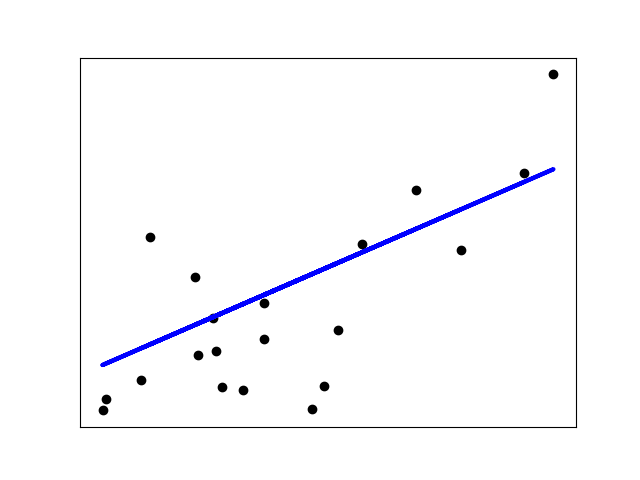
\includegraphics{img/Linear Regression Example.png}
\end{figure}


\section{Non-negative least squares\label{Non-negative least squares}}
In this example, we fit a linear model with positive constraints on the regression coefficients and compare the estimated coefficients to a classic linear regression.

\begin{py}{Non-negative least squares}
import numpy as np
import matplotlib.pyplot as plt
from sklearn.metrics import r2_score
from sklearn.model_selection import train_test_split
from sklearn.linear_model import LinearRegression
np.random.seed(39)

n_samples, n_features = 200, 50
X = np.random.randn(n_samples, n_features)
true_coef = 3 * np.random.randn(n_features)

true_coef[true_coef < 0] = 0
y = np.dot(X, true_coef)
y += 5 * np.random.normal(size=(n_samples, ))

X_train, X_test, y_train, y_test = train_test_split(X, y, test_size=.5)

reg_nnls = LinearRegression(positive=True)
y_pred_nnls = reg_nnls.fit(X_train, y_train).predict(X_test)
r2_score_nnls = r2_score(y_test, y_pred_nnls)
print('NNLS R2 score: {}'.format(r2_score_nnls))

reg_ols = LinearRegression()
y_pred_ols = reg_ols.fit(X_train, y_train).predict(X_test)
r2_score_ols = r2_score(y_test, y_pred_ols)
print('OLS R2 score: {}'.format(r2_score_ols))

fig, ax = plt.subplots()
ax.plot(reg_ols.coef_, reg_nnls.coef_, linewidth=0, marker='.')
low_x, high_x = ax.get_xlim()
low_y, high_y = ax.get_ylim()
low = max(low_x, low_y)
high = min(high_x, high_y)
ax.plot([low, high], [low, high], ls='--', c='.3', alpha=.5)
ax.set_xlabel('OLS regression coefficients', fontweight='bold')
ax.set_ylabel('NNLS regression coefficients', fontweight='bold')
plt.show()
\end{py}

Comparing the regression coefficients between OLS and NNLS, we can observe they are highly correlated (the dashed line is the identity relation), but the non-negative constraint shrinks some to 0. The Non-Negative Least squares inherently yield sparse results.
\begin{figure}
\centering
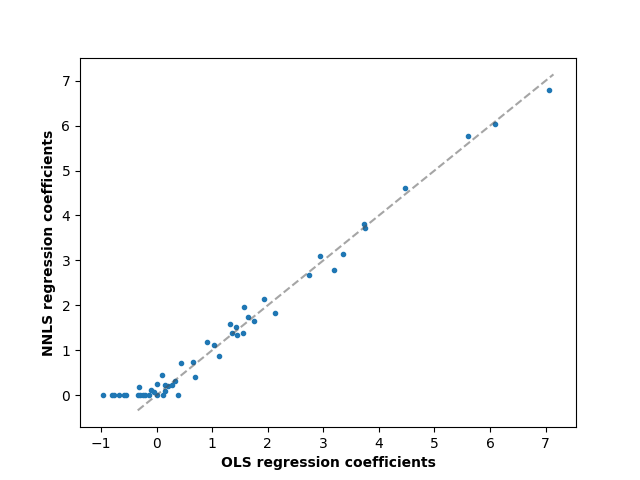
\includegraphics{img/Non-negative least squares.png}

\end{figure}

\section{Plot Ridge coefficients as a function of the regularization\label{Plot Ridge coefficients as a function of the regularization}}
Shows the effect of collinearity in the coefficients of an estimator.

Ridge Regression is the estimator used in this example. Each color represents a different feature of the coefficient vector, and this is displayed as a function of the regularization parameter.

This example also shows the usefulness of applying Ridge regression to highly ill-conditioned matrices. For such matrices, a slight change in the target variable can cause huge variances in the calculated weights. In such cases, it is useful to set a certain regularization (alpha) to reduce this variation (noise).

\textbf{When alpha is very large, the regularization effect dominates the squared loss function and the coefficients tend to zero. At the end of the path, as alpha tends toward zero and the solution tends towards the ordinary least squares, coefficients exhibit big oscillations.} In practise it is necessary to tune alpha in such a way that a balance is maintained between both.

\begin{py}{Ridge coefficients as a function of the regularization}
import numpy as np
import matplotlib.pyplot as plt
from sklearn import linear_model

# X is the 10x10 Hilbert matrix
X = 1.0 / (np.arange(1, 11) + np.arange(0, 10)[:, np.newaxis])
y = np.ones(10)

n_alphas = 200
alphas = np.logspace(-10, -2, n_alphas)
coefs = []
for a in alphas:
    ridge = linear_model.Ridge(alpha=a, fit_intercept=False)
    ridge.fit(X, y)
    coefs.append(ridge.coef_)

ax = plt.gca()
ax.plot(alphas, coefs)
ax.set_xscale("log")
ax.set_xlim(ax.get_xlim()[::-1])
plt.xlabel("alpha")
plt.ylabel("weights")
plt.title("Ridge coefficients as a function of the regularization")
plt.axis("tight")
plt.show()
\end{py}
\begin{figure}
\centering
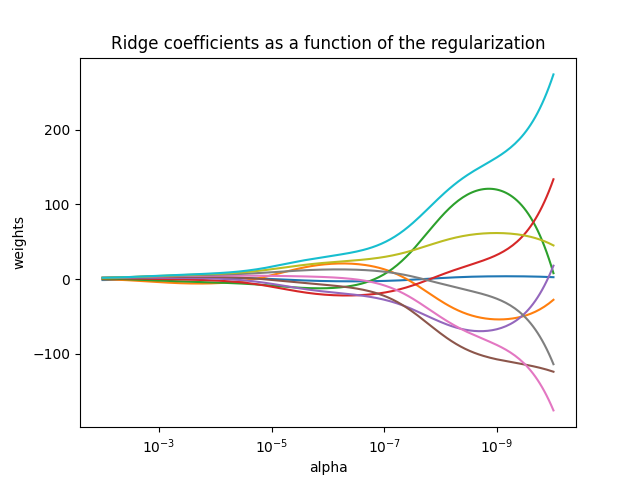
\includegraphics{img/Ridge coefficients as a function of the regularization.png}
\end{figure}

\chapter{Working with text documents\label{Working with text documents}}
\section{Classification of text documents using sparse features\label{Classification of text documents using sparse features}}
This is an example showing how scikit-learn can be used to classify documents by topics using a \href{https://en.wikipedia.org/wiki/Bag-of-words_model}{Bag of Words} approach. This example uses a Tf-idf-weighted document-term sparse matrix to encode the features and demonstrates various classifiers that can efficiently handle sparse matrices.

For document analysis via an unsupervised learning approach, see the example script \nameref{Clustering text documents using k-means}.

\subsection{Loading and vectorizing the 20 newsgroups text dataset\label{Loading and vectorizing the 20 newsgroups text dataset}}

We define a function to load data from The 20 newsgroups text dataset, which comprises around 18,000 newsgroups posts on 20 topics split in two subsets: one for training (or development) and the other one for testing (or for performance evaluation). Note that, by default, the text samples contain some message metadata such as 'headers', 'footers' (signatures) and 'quotes' to other posts. The \verb|fetch_20newsgroups| function therefore accepts a parameter named remove to attempt stripping such information that can make the classification problem “too easy”. This is achieved using simple heuristics that are neither perfect nor standard, hence disabled by default.
\begin{py}{}

\end{py}


\subsection{Analysis of a bag-of-words document classifier}
We will now train a classifier twice, once on the text samples including metadata and once after stripping the metadata. For both cases we will analyze the classification errors on a test set using a confusion matrix and inspect the coefficients that define the classification function of the trained models.
\subsubsection{Model without metadata stripping}
We start by using the custom function \verb|load_dataset| to load the data without metadata stripping.
\begin{minted}{python}
X_train, X_test, y_train, y_test, feature_names, target_names = load_dataset(verbose=True)
\end{minted}
Our first model is an instance of the RidgeClassifier class. This is a linear classification model that uses the mean squared error on \verb|{-1, 1}| encoded targets, one for each possible class. Contrary to LogisticRegression, \textbf{RidgeClassifier does not provide probabilistic predictions} (no \verb|predict_proba| method), \textbf{but it is often faster to train}.

We plot the confusion matrix of this classifier to find if there is a pattern in the classification errors.
\begin{minted}{python}
fig, ax = plt.subplots(figsize=(10, 5))
ConfusionMatrixDisplay.from_predictions(y_test, pred, ax=ax)
ax.xaxis.set_ticklabels(target_names)
ax.yaxis.set_ticklabels(target_names)
ax.set_title('Confusion Matrix for {}\n on thr original documents'.format(clf.__class__.__name__))
plt.show()
\end{minted}
\section{Clustering text documents using k-means\label{Clustering text documents using k-means}}

\section{FeatureHasher and DictVectorizer Comparison\label{FeatureHasher and DictVectorizer Comparison}}

